% document formatting
\documentclass[10pt]{article}
\usepackage[utf8]{inputenc}
\usepackage[left=1in,right=1in,top=1in,bottom=1in]{geometry}
\usepackage[T1]{fontenc}
\usepackage{xcolor}

% math symbols, etc.
\usepackage{amsmath, amsfonts, amssymb, amsthm}

% lists
\usepackage{enumerate}
\usepackage{tabularx}
\usepackage{multicol}

% images
\usepackage{graphicx} % for images

% code blocks
\usepackage{minted, listings} 

% verbatim greek
\usepackage{alphabeta}

\graphicspath{{./assets/images/Week 3}}

\newcommand{\solution}{\textbf{Solution:}} 
\newcommand{\example}{\textbf{Example: }}
\newcommand{\water}{\text{H$_2$O}}
\newcommand{\hydroxide}{\text{OH$^-$}}
\newcommand{\hydronium}{\text{H$_3$O$^+$}}
\newcommand{\proton}{\text{H$^+$}}
\newcommand{\pc}{$^+$}
\newcommand{\nc}{$^-$}
\newcommand{\ka}{\text{$K_\text{a}$}}

\title{CHEM 153A Week 3}

\author{Aidan Jan}
\date{\today}

\begin{document}
\maketitle
\section*{Protein Folding Continued}
\subsection*{More Questions - Levinthal's Paradox}
\begin{itemize}
    \item Other experiments like Anfinsen's raised more questions
    \begin{itemize}
        \item Denatured proteins refold in 0.1-1000 seconds
        \item Take a hypothetical protein with 100 amino acids
        \item Due to allowed rotations, amino acids can have 3 conformations
        \item That's roughly $3^{100}$ possibilities ($\approx 5 \times 10^{47}$)
    \end{itemize}
    \item If the protein can visit one conformation every picosecond ($10^{-12}$ s), searching every possibility would take $5 \times 10^{47} \times 10^{-12}$ seconds, or $1.6 \times 10^{28}$ years.
    \item This is the left diagram
\end{itemize}
\begin{center}
    \includegraphics*[width=\textwidth]{L1_1.png}
\end{center}
\subsection*{The Thermodynamics of Protein Folding}
\begin{itemize}
    \item Free Energy Funnel:
    \begin{itemize}
        \item Unfolded states have high degree of conformational entropy, thus there is high free energy.
        \item The free energy funnel shows that the closer the protein is to its \textbf{native state}, the ideal, lowest energy, folded form, the lower energy it has.
        \begin{itemize}
            \item The middle diagram suggests that there is a pathway guiding the protein folding to the lowest energy state.  This is on the right track, but is not correct.
            \item The right diagram states there are multiple stable intermediates leading to the final folded protein.  This is the most accurate diagram.
        \end{itemize}
    \end{itemize}
\end{itemize}

\subsection*{Hydrophobic Collapse $\rightarrow$ Molten Globule}
\textbf{Hydrophobic collapse} is the rapid burying of hydrophobic residues in the center of the protein - they want to escape their watery environment.
\begin{itemize}
    \item e.g., Val, Leu, Ile, etc.
    \begin{center}
        \includegraphics*[width=\textwidth]{L1_2.png}
    \end{center}
    \item Hydrophobic collapse is entropy-driven: water molecules become more ordered around hydrophobic residues, and the collapse releases that ordered water, increasing entropy.
\end{itemize}
\begin{center}
    \includegraphics*[width=\textwidth]{L1_3.png}
\end{center}
\begin{itemize}
    \item This collapse forms the \textbf{molten globule}, an intermediate transitioning to the final form of the protein
\end{itemize}
\begin{center}
    $\boxed{\includegraphics*[scale=0.5]{L1_4.png}}$
    $\boxed{\includegraphics*[scale=0.35]{L1_5.png}}$
\end{center}
\subsection*{Protein Folding and Energy Landscape}
\begin{center}
    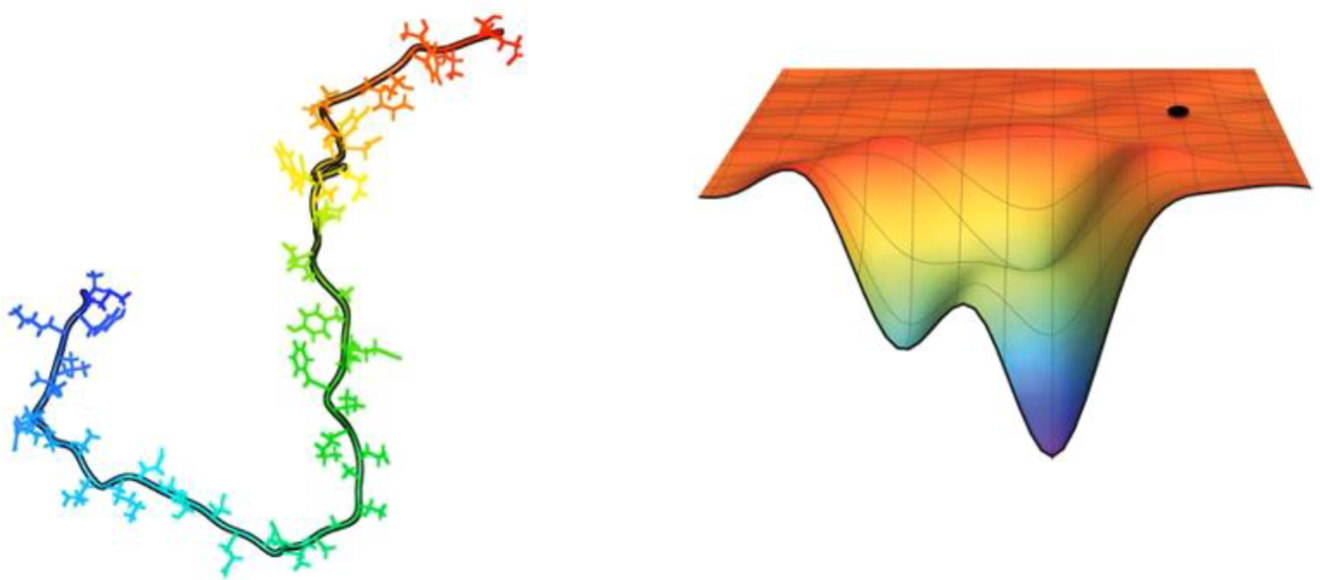
\includegraphics[width=\textwidth]{L1_6.png}
\end{center}
\subsection*{Other Significant Factors in Protein Folding}
\begin{itemize}
    \item \textbf{\underline{Chain conformational entropy}} is the entropy \textit{decrease} due to the formation of an ordered polypeptide
    \item \textbf{\underline{Hydrogen bonding}} serves an important role, mediating interactions with the surrounding water as well as connecting the outer surface of the protein with the hydrophobic core
    \begin{itemize}
        \item They also stabilize interactions between peptide chains (secondary structure)
        \item Enthalpy decrease
    \end{itemize}
    \item \textbf{\underline{London dispersion forces}} hold together the hydrophobic core (enthalpy decrease)
\end{itemize}




\section*{Protein Structures}
\begin{itemize}
    \item \textbf{Protein segments can adopt regular secondary structures such as the $\alpha$ helix and the $\beta$ conformation.}
    \item These structures are defined by particular values of $\phi$ and $\psi$ and their formation is impacted by the amino acid composition on their segment.
    \item All of the $\phi$ and $\psi$ values for a given protein structure can be visualized using a Ramachandran plot.
\end{itemize}

\subsection*{Secondary Structure}
\begin{itemize}
    \item \textbf{secondary structure =} describes the spatial arrangement of the main-chain atoms in a segment of a polypeptide chain
    \begin{itemize}
        \item \textit{regular} secondary structure = $\phi$ and $\psi$ remain the sae throughout the segment
        \item common types = $\alpha$ helix, $\beta$ conformation, $\beta$ turn, random coils
    \end{itemize}
\end{itemize}

\subsubsection*{The $\alpha$ Helix is a Common Protein Secondary Structure}
\begin{itemize}
    \item $\alpha$ helix = simplest arrangement, maximum number of hydrogen bonds
    \begin{itemize}
        \item backbone wound around an imaginary longitudinal axis
        \item R groups protrude out from the backbone
        \item Each helical turn = 3.5 residues, $\sim$5.4 \r{A}
    \end{itemize}
\end{itemize}


\end{document}